\documentclass[12pt,a4paper, oneside]{article}
\usepackage[utf8]{inputenc}
\usepackage[T1]{fontenc}
\usepackage[english,german]{babel}
\usepackage[style=german]{csquotes}
\usepackage{graphicx}

\author{Uni Oldenburg, SWP2020 Gruppe A}
\begin{document}
\begin{titlepage}
\pagestyle{empty}
\begin{center}

\begin{figure}[h]
\centering

\includegraphics[width=0.35\textwidth]{../img/Logo.jpg}
\end{figure}

\bigskip \bigskip \noindent
\textsc{\textbf{\LARGE Softwareprojekt:}} \par \bigskip \noindent
\textsc{\textbf{\LARGE Projekttagebuch}}

\par \bigskip \bigskip \bigskip \bigskip \bigskip \noindent
{\Large Gruppe A} \par \medskip \noindent

\par \bigskip \bigskip \bigskip \bigskip \bigskip \bigskip \noindent
\textit{\Large Wintersemester 2020/21 und} \par \noindent
\textit{\Large Sommersemester 2021}

\par \bigskip \bigskip \bigskip \bigskip \bigskip \bigskip \noindent
\par \bigskip \bigskip \bigskip \noindent
{\Large Sprintanalyse} \par \medskip \noindent

\end{center}
\end{titlepage}

\tableofcontents
\pagebreak

\section{Sprinttagebuch: Sprint-Nr. 11}

\underline{Name des Sprints:}
\\
Sprint 11 Style: Kindergarten

\noindent
\\
\underline{Zeitraum des Sprints:}
\\
27. Mai 2021 - 15. Juni 2021

\noindent
\\
\underline{Ziel des Sprints:}
\\
Insekteneliminierung

\noindent
\\
\underline {Team:}
\\
Sven Ahrens, Alwin Bossert, Aldin Dervisi, Marvin Drees, Mario Fokken, Temmo Junkhoff, Maximilian Lindner, Steven Luong, Phillip-André Suhr, Eric Vuong


\section{Vorgänge}

\begin{itemize}

\item SWP2020A-35: ANmi, dass ein Spieler, der eine Partie vorzeitig verlässt, durch die zufallsbasierte KI ersetzt wird, die für den Spieler übernimmt (2 Story Points)

\item SWP2020A-194: User und Author Objekt aus Messages entfernen und stattdessen "Message.getSession().get().getUser()" nutzen (2 Story Points)

\item SWP2020A-231:	ANmi meine Farbe vor einer Partie anpassen können (2 Story Points)

\item SWP2020A-235: ANmi am Ende einer Partie in einem Graphen sehen können, wer wann wie viele Siegpunkte hatte (2 Story Points)

\item SWP2020A-237: ANmi vor einer Partie zwischen verschiedenen Grafikstilen wählen können (3 Story Points)

\item SWP2020A-256: ANmi statt der config.properties ein Einstellungsmenü nutzen können (4 Story Points)

\item SWP2020A-292: Bericht für Sprint 09 erstellen (2 Story Points)

\item SWP2020A-306:	Clientwechselfunktionalität restlos entfernen (1 Story Point)

\item SWP2020A-330:	ANmi, dass die Dummies in der Gründerphase ihre Startsiedlungen und -straßen bauen (3 Story Point)

\item SWP2020A-339: AEmi, dass die Phasen eines Spielzuges klar organisiert sind und ich angenehm damit arbeiten kann (5 Story Points)

\item SWP2020A-345: ANmin, dass unfaire Täusche getätigt werden (2 Story Points)

\item SWP2020A-346: AEmi keine unnötigen SystemMessageForDingenskirchenMessage haben (1 Story Point)

\item SWP2020A-347: Einigen Buttons u.Ä. fehlen die Sounds (0 Story Points)

\item SWP2020A-348:	AEmi Scene-Wechsel auf Clientseite zentral über einen SceneService steuern können, damit XPresenter nicht immer selbst auf den EventBus posten (2 Story Points)

\item SWP2020A-349:	Nach dem Bezahlen des Robber-Tax sind manchmal die Ressourcen im Minus-Bereich (2 Story Points)

\item SWP2020A-351: ANmi, dass sich das Gegenangebotsfenster beim ursprünglich angefragten Nutzer schließt, wenn der aktive Spieler dessen Gegenangebot ablehnt (1 Story Point)

\item SWP2020A-352:	ANmi die Hilfetexte auch bei dunklem Hintergrund und maximiertem Fenster lesen können (1 Story Point)

\item SWP2020A-355:	ANmi gewisse Chatkommandos, die nicht Cheats beinhalten, nutzen können (2 Story Points)

\item SWP2020A-357:	Bericht für Sprint 10 erstellen (2 Story Points)

\item SWP2020A-358:	AEmi, dass alle wichtigen Codesegmente durch Tests abgedeckt sind (5 Story Points)

\item SWP2020A-360:	Die Chat-Systemnachricht wird beim Entfernen bzw. Auflösung einer Lobby nicht korrekt angezeigt (0 Story Points)

\item SWP2020A-361: ANmi, dass die KI in der Gründungsphase baut (2 Story Points)

\item SWP2020A-362:	AEmi, dass die KI Methoden getestet werden (2 Story Points)

\item SWP2020A-363:	AEmi, dass die JavaDocs einiger Methoden in AbstractPresenterWithChatWithGameWithPreGamePhase mit ihrer Funktionen übereinstimmen (0 Story Points)

\item SWP2020A-365: ANmi, dass die Reihenfolge der Spieler in der Spielerliste der Spielreihenfolge entspricht (1 Story Point)

\item SWP2020A-366:	ANmi/ AEmi nicht überall ein hohes Risiko für NullPointerExceptions haben (2 Story Points)

\item SWP2020A-369: ANmi, dass ich bei der Registrierung immer nur einen Namen eingeben kann, der den Einschränkungen der Entwickler entspricht (0 Story Points)

\item SWP2020A-370:	LOG-Einträge sollten nicht vom ThreadManager verlagert werden (1 Story Point)

\item SWP2020A-371:	PGCanvas Invalid Token \& Falsche Farben beim Zeichnen auf den Canvas (0 Story Points)

\item SWP2020A-372:	ANmi, dass die Anzeige des aktuellen Spieler immer auch dem Spieler entspricht, der aktuell am Zug ist (1 Story Point)

\item SWP2020A-373:	ANmi, dass das Handelsfenster (schon wieder) korrekt funktioniert (1 Story Point)

\item SWP2020A-374:	ANmi das Lobbyfenster verlässlich schließen können (1 Story Point)

\item SWP2020A-375:	ANmi, dass ich nur in einer Art Baumodus auf das Spielfeld bauen kann, welchen ich mit einer Checkbox o.Ä. aktivieren muss (1 Story Point)

\item SWP2020A-376:	Horizontales Scrollen im Chat (erneut) deaktivieren (0 Story Points)

\item SWP2020A-378: Zug beendbar bevor der Räuber verschoben wurde, nachdem man Tax bezahlt hat (1 Story Point)

\item SWP2020A-379: AEmi Guice nicht per FieldInjection nutzen (1 Story Point)
\end{itemize}

\newpage

\subsection{Sprinterfolg}

\begin{figure}[h]
    \centering
   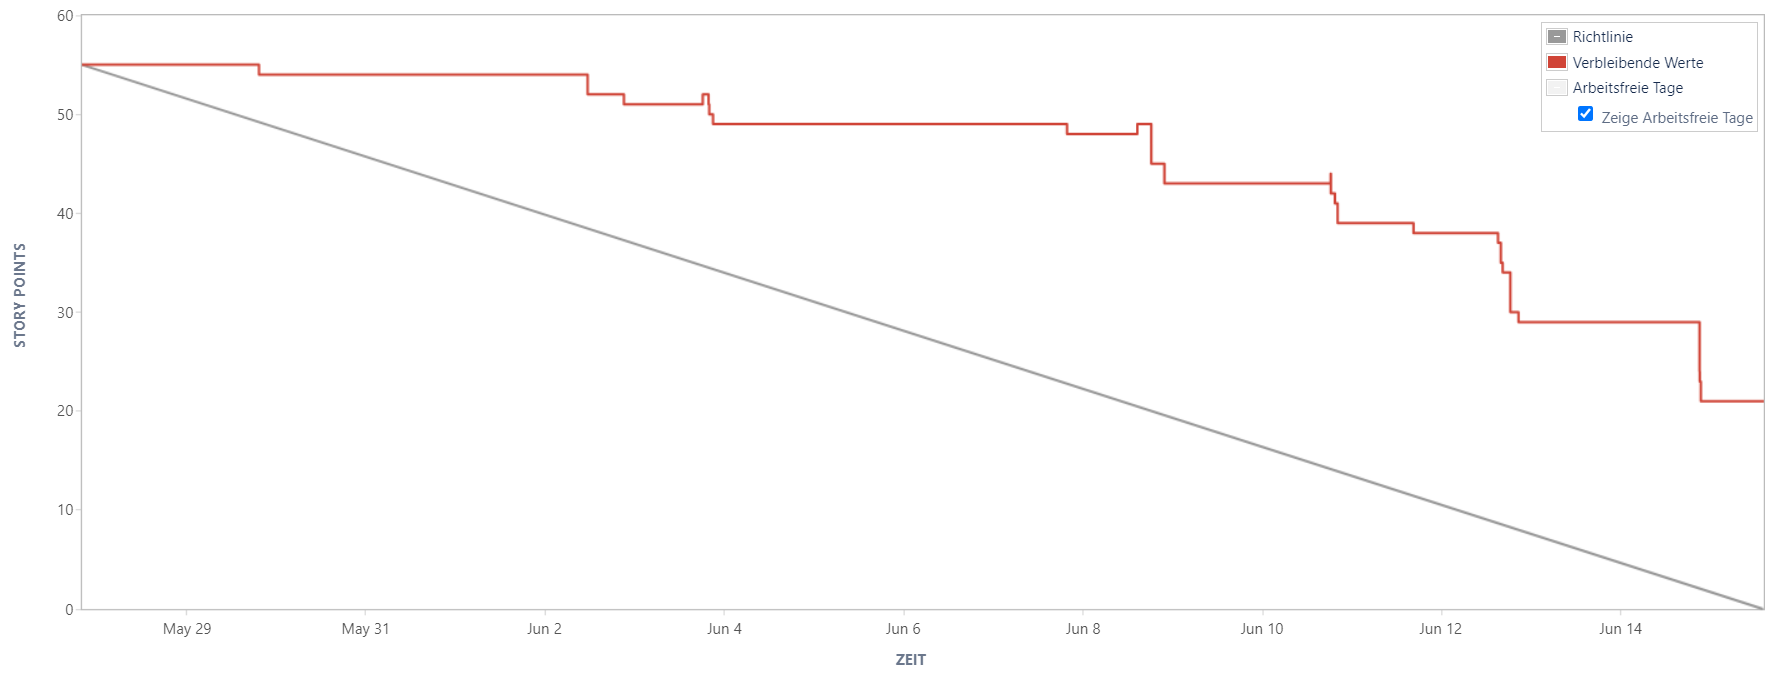
\includegraphics[width=\textwidth, height=5cm]{../img/sprint_11/Burndown-Sprint11.png}
    \caption{Burndown-Diagramm Sprint 11}
    \label{fig: Burndown-Sprint 11}
\end{figure}

\noindent
Der Sprint 11 war bisher nach Sprint 01 einer der schwächsten Sprints unseres Softwareprojektes im Bezug auf der geleisteten Leistung im Vergleich
zu den gesetzten Story Points. Am Beginn des Sprints betrug die Höhe der Story Points einen Gesamtaufwand von 55 Story Points.
Aus dem Burndown-Diagramm wird ersichtlich, dass im frühem Verlauf die Arbeitsaktivität sehr gering war und sich dies bis zum mittleren
Zeitraum des Sprints kaum verändert hat. Es wurden bis zum 08. Juni lediglich 6 Story Points abgeschlossen, was deutlich sichtbar macht, dass in den
ersten 1 1/2 Wochen sehr geringe bis keine Fortschritte in diesem Sprint getätigt wurden. Erst in den letzten Tagen bzw. im letzten Sprintzeitraum
wurden die meisten Tasks abgeschlossen bzw. in PR gestellt.
Des Weiteren wurden folgende Tasks nachgezogen: \textit{SWP2020A-378: Zug beendbar bevor der Räuber verschoben wurde, nachdem man Tax bezahlt hat (1 Story Point), SWP2020A-347: Einigen Buttons u.Ä. fehlen die Sounds (0 Story Points), SWP2020A-379: AEmi Guice nicht per FieldInjection nutzen (1 Story Point)}.
Schlussendlich wurden lediglich 34 von 55 Story Points am 15. Juni 2021 erfolgreich abgeschlossen und die nicht fertiggestellten Tasks,
wurden in den nächsten Sprint gezogen.

\newpage

\subsection{Sprintprobleme bzw. Hindernisse}

Zum Anfang des Sprints am 27. Mai 2021 bis hin zum 08. Juni 2021 wies das Team kaum Fortschritte vor im Bezug auf
abgeschlossene Tasks. Zwar wurden im Verlauf des Sprints immer wieder 0-Punkte-Tasks abgeschlossen, jedoch wurde
dementsprechend auch kein Burndown verzeichnet. Weiterhin wurde aufgrund der Ansammlung vieler Tasks in PR ersichtlich, dass viele Reviews definitv
zu lang gebraucht haben und infolgedessen viele Tasks lange in Review standen.
Dies führte dementsprechend auch zu einem niedrigen Abschlussverzeichnis im Burndown-Diagramm.
Des Weiteren wird in diesem Sprint das immer wiederkehrende Problem des Zeitmanagements ersichtlich, das zu unabgeschlossenen Tasks führt.
Viele Tasks wurden erst gegen Ende des Sprints abgeschlossen sprich angefangen, was defintiv zu einer schwachen Leistung innerhalb eines Sprints
resultiert. Kommt es zu unerwarteten Problemen oder Verschätzungen des Aufwands einer oder mehrerer Tasks, kann es dazu führen, dass Tasks nicht
rechtzeitig abgeschlossen werden können. Folglich wurden in diesem Sprint folgende Tasks nicht zeitgerecht abgeschlossen:

\begin{itemize}
    \item SWP2020A-35: ANmi, dass ein Spieler, der eine Partie vorzeitig verlässt, durch die zufallsbasierte KI ersetzt wird, die für den Spieler übernimmt (2 Story Points)

    \item SWP2020A-194: User und Author Objekt aus Messages entfernen und stattdessen "Message.getSession().get().getUser()" nutzen (2 Story Points)

    \item SWP2020A-235: ANmi am Ende einer Partie in einem Graphen sehen können, wer wann wie viele Siegpunkte hatte (2 Story Points)

    \item SWP2020A-237: ANmi vor einer Partie zwischen verschiedenen Grafikstilen wählen können (3 Story Points)

    \item SWP2020A-330:	ANmi, dass die Dummies in der Gründerphase ihre Startsiedlungen und -straßen bauen (3 Story Point)

    \item SWP2020A-339: AEmi, dass die Phasen eines Spielzuges klar organisiert sind und ich angenehm damit arbeiten kann (5 Story Points)

    \item SWP2020A-348:	AEmi Scene-Wechsel auf Clientseite zentral über einen SceneService steuern können, damit XPresenter nicht immer selbst auf den EventBus posten (2 Story Points)

    \item SWP2020A-355:	ANmi gewisse Chatkommandos, die nicht Cheats beinhalten, nutzen können (2 Story Points)
\end{itemize}


\section{Erkenntnis aus der Retrospektive}

Folgende Erkenntnisse ergaben sich aus der Retrospektive:
\\

\underline{Start:}

\begin{itemize}
    \item Vorgangslite bei jedem Meeting durchgehen
    \item Tests schreiben
    \item Bei Problemen einfach fragen
    \item Lebenszeichenkontrolle nach ungewöhnlich langer Inaktivität
\end{itemize}

\underline{Stop:}

\begin{itemize}
    \item Wenn in den Meetings was zu den eigenen Tasks besprochen wird, sollte man das nicht einfach ignorieren, sondern merken/ aufschreiben und einarbeiten
    \item Tasks mindestens einen Punkt geben
    \item Reviews sollten nach spätestens 48 Stunden erledigt sein
    \item Frühzeitig Reviews durchführen
    \item Reviewumverteilung nach 48 Stunden
\end{itemize}

\underline{Weiter so:}

\begin{itemize}
    \item Kleine Tasks machen oder große frühzeitig aufteilen, sollte man merken, dass es zu viel wird
    \item Discord Verfügbarkeit beibehalten
    \item Gründliche Reviews
\end{itemize}

\newpage

\section{Sonstige Anmerkungen}

Was deutlich anzumerken war in diesem Sprint ist das Aufschieben von Tasks und das negative Zeitmanagement.
Ebenfalls zu erwähnen, die relativ langsamen Reviews und die folgliche Anstauung von PRs.
Im Verlauf der letzten Sprints lässt sich erkennen, dass die starke Reduzierung von Pair-Programming deutlich die generelle Leistung der gesamten
Gruppe negativ beeinflusst hat, wobei man sagen muss, dass Solo-Programming als auch Pair-Programming ihre Vor- und Nachteile haben.
Des Weiteren wurde beschlossen, dass keine Tasks mehr mit 0 Story Points versehen werden sollten, sodass mindestens ein Fortschritt im
Burndown-Diagramm zu verzeichnen ist. Weiterhin wurde ebenfalls beschlossen, dass zu jedem Meeting eine kurze Fortschrittsbesprechung zu jedem
Vorgang abgegeben werden muss.

\section{Fazit}

Grundsätzlich lässt sich sagen, dass in diesem Sprint die Gesamtleistung aufgrund von unterschiedlichen Problemen wie Zeitmanagement, Reviewdauer etc.
nicht unserem gewünschtem Ergebnis entsprach. Unser Sprintziel der Bug-Entfernung wurden teils erfüllt, aber es sind immer noch viele Bugs
aufzuklären und zu lösen. Des Weiteren befinden wir uns nun in der Endphase des Software-Projektes, wobei wir uns jetzt vorallem in unserem letzten
Sprint-Marathon auf die Testabdeckung, Prüfung und Optimierung der Qualität des Codes sowie auch auf Dokumentation und Bug-Eliminierung konzentrieren
sollten, sodass wir am Ende unser Projekt erfolgreich übergeben können.

\end{document}